\subsection{ProteomicsDB: protein-level detection in normal tissues}
\label{sec:proteomicsdb}
Gated antigens were chosen for tumour-restricted RNA expression. We asked
whether mass spectrometry agrees at the protein level. For each study gene we
mapped the UniProt accession to its ProteomicsDB target protein and retrieved
every protein-expression row, then joined the sample table (tissue, species,
disease). A normal-tissue sample was defined before any group comparison as
human, disease-free, and in a fixed whitelist of 75 organ and tissue names.

\paragraph{Calibration gate.} Pre-registered gates PASSED: (G1) 196 of
205 genes mapped to a ProteomicsDB target protein (threshold 180);
(G2) CD19 detected in 344 B-lineage samples (threshold 1); (G3) all four
housekeeping controls detected in at least ten normal tissues (minimum
observed 37).
\paragraph{Hypothesis H1 (falsified, reversed).} H1 predicted that gated
proteins are detected in fewer distinct normal tissues than background
(one-sided test).
The opposite holds: median 20 versus 5 normal tissues
(one-sided $p=1$). Gated genes are also detected in some sample more
often (97/98 versus 74/90, Fisher $p=4.3\times10^{-5}$).

\paragraph{Control H3.} Background contains proteins that mass spectrometry
rarely sees (immunoglobulin and T-cell receptor segments, olfactory
receptors), so the reversal could be detectability alone.
Restricting to genes detected in at least one sample (declared after H1),
the gated excess remains: median 21 versus 7.5 normal tissues
(97 gated, 74 background; two-sided $p=8.1\times10^{-6}$).
Mass spectrometry does not confirm the RNA-level restriction: gated proteins are seen in more normal human tissues than background, and the excess survives the detectability control. Protein-level off-tumour exposure therefore needs per-antigen review rather than being assumed from RNA windows.

\paragraph{AND-gate antigens.} normal tissues with detection: CA9 7 tissues; CA12 27 tissues; CLDN18 6 tissues; CLDN6 1 tissues; MSLN 19 tissues; PSCA 6 tissues; SLC39A6 15 tissues.

\begin{figure}[t]
\centering
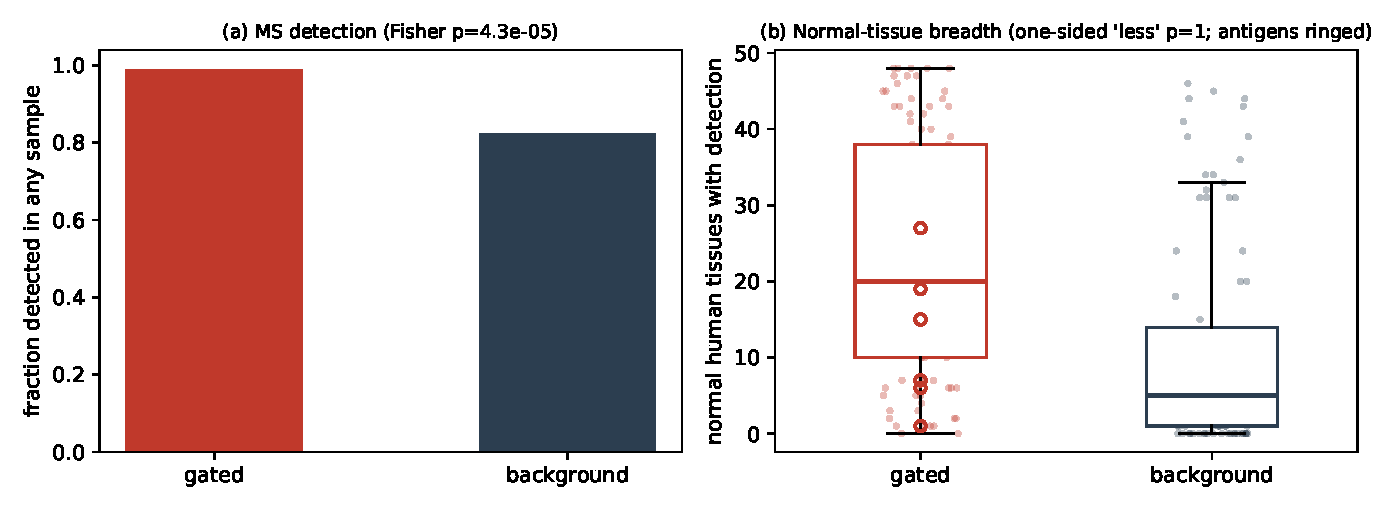
\includegraphics[width=\linewidth]{proteomicsdb_fig.pdf}
\caption{ProteomicsDB protein-level audit. (a) Fraction of mapped genes
detected by mass spectrometry in any sample. (b) Distinct normal human
tissues with detection per gene; AND-gate antigens ringed.}
\label{fig:proteomicsdb}
\end{figure}
